\chapter{闵可夫斯基时空与洛伦兹协变性}

\section{狭义相对论的基本原理}

牛顿力学把时间和空间看作彼此独立的结构。时间作为统一的外部参数流逝，空间则是三维欧氏空间。这种时空观在低速运动中给出良好的近似，但当物体速度接近光速时，时间间隔、空间长度以及同时性都不再具有牛顿意义下的绝对性。狭义相对论正是在这种背景下建立起来的时空理论。

狭义相对论基于两个基本原理。第一是相对性原理：所有惯性参考系中，物理规律具有相同形式。第二是光速不变原理：真空中的光速在所有惯性参考系中相同，与光源和观察者的运动状态无关。

这两个原理要求重新理解时间和空间的关系。在相对论中，时间和空间不再是彼此分离的对象，而是共同组成四维时空。一个在某一时刻、某一地点发生的物理事实称为一个事件。确定一个事件需要一个时间坐标和三个空间坐标，通常写为
\begin{equation}
\label{eq:ch5-event-coordinate}
x^{\mu}=(x^{0},x^{1},x^{2},x^{3})=(ct,x,y,z).
\end{equation}
\eqref{eq:ch5-event-coordinate} 中希腊指标 $\mu,\nu,\rho,\sigma$ 的取值为 $0,1,2,3$，表示四维时空指标；拉丁指标 $i,j,k$ 的取值为 $1,2,3$，表示三维空间指标。取 $x^{0}=ct$ 的原因是使时间分量与空间分量具有相同的长度量纲。

在本章中，三维空间矢量用粗体表示，例如 $\bm{r},\bm{v},\bm{p}$；四维对象主要用指标表示，例如 $x^{\mu},A^{\mu},T^{\mu\nu}$。这种记号区分有助于避免三维欧氏结构与四维闵可夫斯基结构之间的混淆。

\section{事件、世界线与时空间隔}

在四维时空中，粒子的运动不再仅仅是三维空间中的轨迹，而是一条四维曲线。这条曲线称为世界线。若粒子在某一惯性系中的空间位置为
\[
\bm{r}=\bm{r}(t),
\]
则其世界线可写为
\[
x^{\mu}(t)=(ct,\bm{r}(t)).
\]
世界线上的每一点对应一个事件，而整条世界线描述粒子在时空中的完整历史。
\begin{figure}
	\centering
	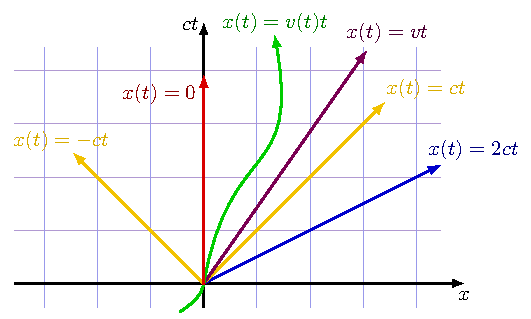
\includegraphics[width=0.6\linewidth]{figure/fig5.1}
	\caption[几条速度不同的时空世界线]{几条速度不同的时空世界线}
	\label{fig:5.1}
\end{figure}

对于两个无限接近的事件，坐标差为
\[
\dif x^{\mu}=(c\dif t,\dif x,\dif y,\dif z).
\]
狭义相对论中的基本几何量不是四维欧氏距离，而是闵可夫斯基时空间隔：
\begin{equation}
\label{eq:ch5-spacetime-interval}
\dif s^{2}=c^{2}\dif t^{2}-\dif x^{2}-\dif y^{2}-\dif z^{2}.
\end{equation}
该表达式中，时间项与空间项具有相反符号。这一点是相对论时空区别于欧氏空间的根本特征。

真空中的光信号满足
\[
\dif x^{2}+\dif y^{2}+\dif z^{2}=c^{2}\dif t^{2},
\]
因此光信号连接的两个无限接近事件满足
\[
\dif s^{2}=0.
\]
光速不变原理要求：若一个惯性系中某段间隔为零，则所有惯性系中该间隔仍为零。更强地，洛伦兹变换保持整个时空间隔 $\dif s^{2}$ 不变。

根据 \eqref{eq:ch5-spacetime-interval} 中 $\dif s^{2}$ 的符号，时空间隔分为三类。若
\[
\dif s^{2}>0,
\]
称为类时间隔；若
\[
\dif s^{2}=0,
\]
称为类光间隔；若
\[
\dif s^{2}<0,
\]
称为类空间隔。类光方向组成光锥。光锥内部是类时区域，其中事件之间可以存在因果联系；光锥外部是类空区域，其中事件之间不能通过速度不超过光速的信号建立因果联系。
\begin{figure}
	\centering
	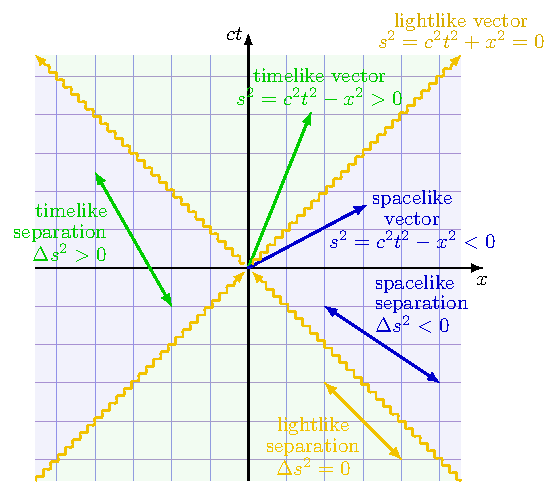
\includegraphics[width=0.6\linewidth]{figure/fig5.2}
	\caption[不同类型的时空矢量和分离]{不同类型的时空矢量和分离}
	\label{fig:5.2}
\end{figure}

\section{闵可夫斯基度规与指标升降}

为了把时空间隔写成张量形式，引入闵可夫斯基度规 $\eta_{\mu\nu}$。本讲义采用号差约定
\begin{equation}
\label{eq:ch5-minkowski-metric}
\eta_{\mu\nu}=\mathrm{diag}(1,-1,-1,-1).
\end{equation}
由 \eqref{eq:ch5-minkowski-metric}，时空间隔可写为
\begin{equation}
\label{eq:ch5-interval-tensor-form}
\dif s^{2}=\eta_{\mu\nu}\dif x^{\mu}\dif x^{\nu}.
\end{equation}
\eqref{eq:ch5-interval-tensor-form} 展开即为
\[
\dif s^{2}=(\dif x^{0})^{2}-(\dif x^{1})^{2}-(\dif x^{2})^{2}-(\dif x^{3})^{2},
\]
由 $x^{0}=ct$ 可得
\[
\dif s^{2}=c^{2}\dif t^{2}-\dif x^{2}-\dif y^{2}-\dif z^{2}.
\]

闵可夫斯基度规的逆矩阵记为 $\eta^{\mu\nu}$。在当前惯性坐标和号差约定下，
\[
\eta^{\mu\nu}=\mathrm{diag}(1,-1,-1,-1),
\]
并满足
\begin{equation}
\label{eq:ch5-metric-inverse}
\eta^{\mu\alpha}\eta_{\alpha\nu}=\delta^{\mu}{}_{\nu}.
\end{equation}
\eqref{eq:ch5-metric-inverse} 表示 $\eta^{\mu\nu}$ 是 $\eta_{\mu\nu}$ 的逆矩阵。

度规可以降低指标。若 $A^{\mu}$ 是反变四维矢量，则其协变分量定义为
\begin{equation}
\label{eq:ch5-lower-index}
A_{\mu}=\eta_{\mu\nu}A^{\nu}.
\end{equation}
于是
\[
A_{0}=A^{0},\qquad A_{i}=-A^{i}.
\]
若把四维矢量写为
\[
A^{\mu}=(A^{0},\bm{A}),
\]
则对应的协变形式为
\[
A_{\mu}=(A^{0},-\bm{A}).
\]
反过来，升高指标由
\begin{equation}
\label{eq:ch5-raise-index}
A^{\mu}=\eta^{\mu\nu}A_{\nu}
\end{equation}
给出。\eqref{eq:ch5-lower-index} 与 \eqref{eq:ch5-raise-index} 是闵可夫斯基度规升降指标的基本规则。

两个四维矢量的闵可夫斯基内积为
\begin{equation}
\label{eq:ch5-minkowski-inner-product}
A^{\mu} B_{\mu}=\eta_{\mu\nu}A^{\mu} B^{\nu}.
\end{equation}
\eqref{eq:ch5-minkowski-inner-product} 展开得
\[
A^{\mu} B_{\mu}=A^{0}B^{0}-A^{1}B^{1}-A^{2}B^{2}-A^{3}B^{3}
=A^{0}B^{0}-\bm{A}\cdot\bm{B}.
\]
特别地，
\[
A^{\mu} A_{\mu}=(A^{0})^{2}-\bm{A}^{2}.
\]
该量由 \eqref{eq:ch5-minkowski-inner-product} 得到，在洛伦兹变换下保持不变，因此称为洛伦兹标量。

\section{固有时与类时世界线}

对于类时世界线，可以选取随粒子一起运动的瞬时惯性系。在该瞬时静止系中，粒子的空间坐标不变，即
\[
\dif x=\dif y=\dif z=0.
\]
此时随粒子一起运动的时钟记录的时间称为固有时，记为 $\tau$。在瞬时静止系中有
\begin{equation}
\label{eq:ch5-proper-time-interval}
\dif s^{2}=c^{2}\dif\tau^{2}.
\end{equation}
而在一般实验室系中，同一段世界线元满足
\[
\dif s^{2}=c^{2}\dif t^{2}-(\dif x^{2}+\dif y^{2}+\dif z^{2}).
\]
由于 $\dif s^{2}$ 是洛伦兹不变量，\eqref{eq:ch5-proper-time-interval} 与实验室系表达式相等：
\[
c^{2}\dif\tau^{2}=c^{2}\dif t^{2}-(\dif x^{2}+\dif y^{2}+\dif z^{2}).
\]
令三维速度为
\[
\bm{v}=\frac{\dif\bm{r}}{\dif t},
\qquad
v^{2}=\frac{\dif x^{2}+\dif y^{2}+\dif z^{2}}{\dif t^{2}},
\]
则有
\begin{equation}
\label{eq:ch5-proper-time}
\dif\tau=\dif t\sqrt{1-\frac{v^{2}}{c^{2}}}.
\end{equation}
定义洛伦兹因子
\begin{equation}
\label{eq:ch5-lorentz-factor}
\gamma=\frac{1}{\sqrt{1-\frac{v^{2}}{c^{2}}}},
\end{equation}
于是
\[
\dif t=\gamma\dif\tau.
\]
由 \eqref{eq:ch5-proper-time} 和 \eqref{eq:ch5-lorentz-factor} 可见，在实验室系看来，运动时钟经历的固有时间小于实验室时间，即运动时钟变慢。

固有时的几何意义在于：它是类时世界线的自然参数。对类时世界线，有
\[
\dif\tau=\frac{1}{c}\sqrt{\eta_{\mu\nu}\dif x^{\mu}\dif x^{\nu}}.
\]
因此，固有时不是某个外部参考系中的普通时间，而是沿粒子自身世界线测得的时间。下一章将以固有时为参数定义四速度、四动量和相对论动力学方程。


\section{洛伦兹群}

前面已经看到，闵可夫斯基时空间隔由度规 $\eta_{\mu\nu}$ 给出。若一个线性变换保持该间隔不变，就应满足
\[
\eta_{\mu\nu}x'^{\mu}x'^{\nu}
=
\eta_{\mu\nu}x^{\mu}x^{\nu}.
\]
设四维坐标按
\[
x'^{\mu}
=
\Lambda^{\mu}{}_{\nu}x^{\nu}
\]
变换。代入上式，得到
\[
\eta_{\mu\nu}
\Lambda^{\mu}{}_{\alpha}
\Lambda^{\nu}{}_{\beta}
x^{\alpha}x^{\beta}
=
\eta_{\alpha\beta}x^{\alpha}x^{\beta}.
\]
由于该关系对任意四维坐标 $x^{\alpha}$ 成立，必须有
\begin{equation}
\label{eq:ch5-lorentz-condition-index}
\eta_{\mu\nu}
\Lambda^{\mu}{}_{\alpha}
\Lambda^{\nu}{}_{\beta}
=
\eta_{\alpha\beta}.
\end{equation}
\eqref{eq:ch5-lorentz-condition-index} 用矩阵记号可写为
\begin{equation}
\label{eq:ch5-lorentz-condition}
\Lambda^{T}\eta\Lambda
=
\eta.
\end{equation}
\eqref{eq:ch5-lorentz-condition} 就是洛伦兹变换的定义条件。

所有满足上述条件的实四维线性变换组成洛伦兹群：
\begin{equation}
\label{eq:ch5-lorentz-group}
O(1,3)
=
\{\Lambda\in GL(4,\mathbb{R})\mid \Lambda^{T}\eta\Lambda=\eta\}.
\end{equation}
这里的符号 $O(1,3)$ 表示 \eqref{eq:ch5-lorentz-group} 中的群保持一个号差为 $(1,3)$ 的二次型不变。它可以看作闵可夫斯基度规下的正交群，与欧氏空间中保持 $\delta_{ij}$ 不变的正交群 $O(3)$ 平行。

由定义式 \eqref{eq:ch5-lorentz-condition} 两边取行列式，得
\[
\det(\Lambda^{T})\det(\eta)\det(\Lambda)
=
\det(\eta).
\]
由于 $\det(\Lambda^{T})=\det(\Lambda)$，且 $\det(\eta)\neq 0$，因此
\[
(\det\Lambda)^{2}=1.
\]
所以
\[
\det\Lambda=\pm 1.
\]
这说明洛伦兹群包含保持空间取向的部分和反转空间取向的部分。

洛伦兹群还可以按是否保持时间方向分为不同连通分支。物理中最常用的是既保持空间取向又保持时间方向的分支，称为正时固有洛伦兹群，记为
\[
SO^{+}(1,3).
\]
其中 “固有” 对应 $\det\Lambda=1$，“正时” 对应时间方向不反转。

洛伦兹群包含两类基本连续变换。一类是普通空间旋转，它只混合空间坐标而不混合时间坐标；另一类是 boost，它混合时间坐标与空间坐标。下一节讨论的沿一维方向的洛伦兹变换就是最简单的 boost。

\section{洛伦兹变换}

洛伦兹变换是保持闵可夫斯基时空间隔不变的线性变换。设一个惯性系 $K'$ 相对于惯性系 $K$ 沿 $+x$ 方向以速度 $V$ 匀速运动，并且在 $t=t'=0$ 时两个坐标系原点重合。本讲义约定 $K'$ 的原点在 $K$ 中满足
\[
x=Vt.
\]
从 $K'$ 到 $K$ 的洛伦兹变换为
\[
x=\gamma(x'+Vt'),
\]
\[
t=\gamma\left(t'+\frac{V}{c^{2}}x'\right),
\]
以及
\[
y=y',\qquad z=z'.
\]
其中
\begin{equation}
\label{eq:ch5-boost-gamma}
\gamma=\frac{1}{\sqrt{1-\frac{V^{2}}{c^{2}}}}.
\end{equation}
\eqref{eq:ch5-boost-gamma} 是该相对速度对应的洛伦兹因子。写成四维列向量形式为
\begin{equation}
\label{eq:ch5-standard-boost}
\begin{pmatrix}
	ct\\x\\y\\z
\end{pmatrix}
=
\begin{pmatrix}
	\gamma & \gamma\frac{V}{c} & 0 & 0\\
	\gamma\frac{V}{c} & \gamma & 0 & 0\\
	0&0&1&0\\
	0&0&0&1
\end{pmatrix}
\begin{pmatrix}
	ct'\\x'\\y'\\z'
\end{pmatrix}.
\end{equation}
\eqref{eq:ch5-standard-boost} 对应的逆变换为
\[
x'=\gamma(x-Vt),
\]
\[
t'=\gamma\left(t-\frac{V}{c^{2}}x\right),
\]
以及
\[
y'=y,
\qquad
z'=z.
\]
矩阵形式为
\begin{equation}
\label{eq:ch5-inverse-boost}
\begin{pmatrix}
	ct'\\x'\\y'\\z'
\end{pmatrix}
=
\begin{pmatrix}
	\gamma & -\gamma\frac{V}{c} & 0 & 0\\
	-\gamma\frac{V}{c} & \gamma & 0 & 0\\
	0&0&1&0\\
	0&0&0&1
\end{pmatrix}
\begin{pmatrix}
	ct\\x\\y\\z
\end{pmatrix}.
\end{equation}
\eqref{eq:ch5-inverse-boost} 可由 \eqref{eq:ch5-standard-boost} 中令 $V\to -V$ 得到。
\begin{figure}
	\centering
	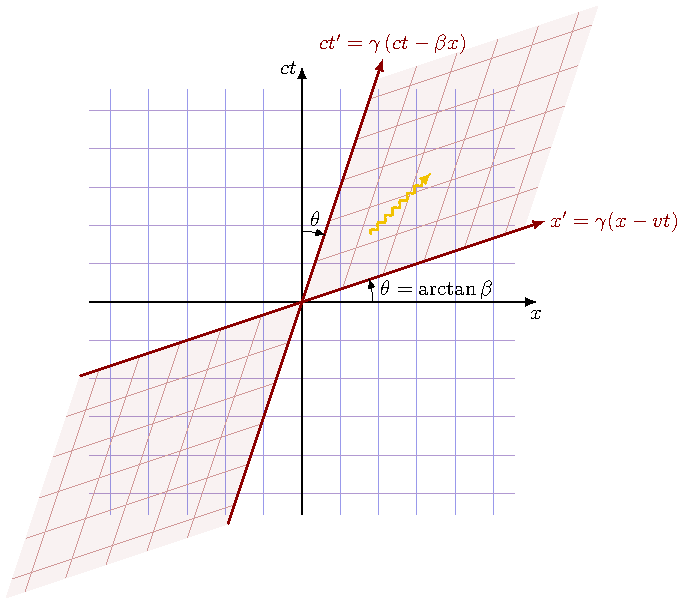
\includegraphics[width=0.5\linewidth]{figure/fig5.3}
	\caption[洛伦兹变换]{洛伦兹变换}
	\label{fig:5.3}
\end{figure}


更一般地，设洛伦兹变换写成
\[
x'^{\mu}=\Lambda^{\mu}{}_{\nu} x^{\nu}.
\]
保持闵可夫斯基度规不变要求
\begin{equation}
\label{eq:ch5-lorentz-condition-alt}
\eta_{\alpha\beta}\Lambda^{\alpha}{}_{\mu}\Lambda^{\beta}{}_{\nu}=\eta_{\mu\nu}.
\end{equation}
\eqref{eq:ch5-lorentz-condition-alt} 的矩阵形式为 \eqref{eq:ch5-lorentz-condition}。
\eqref{eq:ch5-lorentz-condition-alt} 等价地给出了洛伦兹群 \eqref{eq:ch5-lorentz-group}。
由该条件取行列式，可得
\[
(\det\Lambda)^{2}=1,
\]
即
\[
\det\Lambda=\pm 1.
\]
物理中常用的是保持空间取向和时间方向的正时固有洛伦兹群 $SO^{+}(1,3)$。

\section{洛伦兹变换的双曲旋转形式}

洛伦兹变换的几何结构在二维闵可夫斯基平面中最为清楚。只考虑 $(ct,x)$ 平面，间隔不变要求
\[
(ct)^{2}-x^{2}=(ct')^{2}-x'^{2}.
\]
\begin{figure}[h]
	\centering
	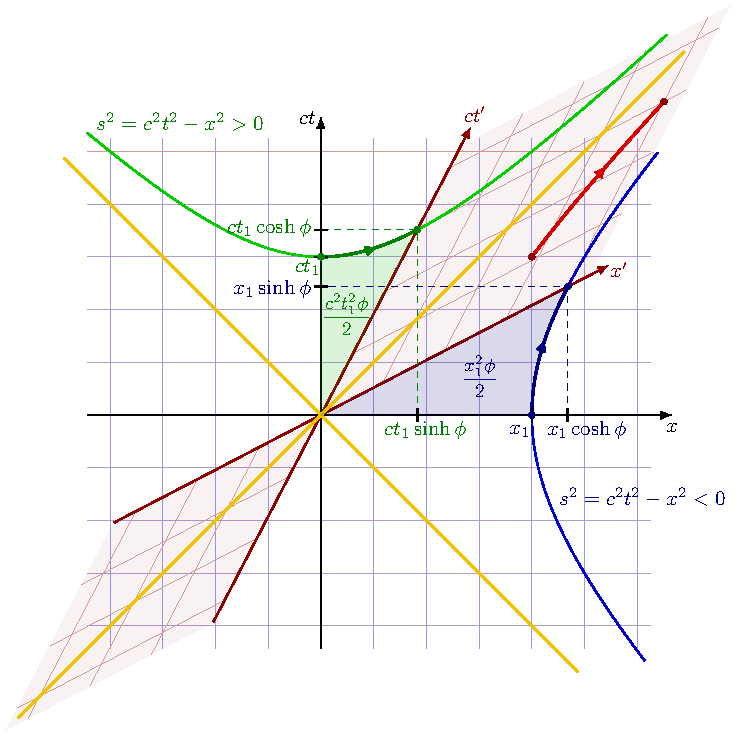
\includegraphics[width=0.7\linewidth]{figure/fig5.4}
	\caption[闵可夫斯基时空中的双曲线]{闵可夫斯基时空中的双曲线}
	\label{fig:5.4}
\end{figure}

保持平方差不变的线性变换可以写成双曲旋转：
\begin{equation}
\label{eq:ch5-hyperbolic-boost}
\begin{pmatrix}
	ct\\x
\end{pmatrix}
=
\begin{pmatrix}
	\cosh\theta&\sinh\theta\\
	\sinh\theta&\cosh\theta
\end{pmatrix}
\begin{pmatrix}
	ct'\\x'
\end{pmatrix}.
\end{equation}
\eqref{eq:ch5-hyperbolic-boost} 展开得
\[
ct=ct'\cosh\theta+x'\sinh\theta,
\]
\[
x=ct'\sinh\theta+x'\cosh\theta.
\]
由于双曲函数满足
\[
\cosh^{2}\theta-\sinh^{2}\theta=1,
\]
故该变换保持 $(ct)^{2}-x^{2}$ 不变。

参数 $\theta$ 称为快度。考察 $K'$ 的原点，其在 $K'$ 中满足 $x'=0$。代入上式得
\[
x=ct'\sinh\theta,
\qquad
ct=ct'\cosh\theta.
\]
因此该原点在 $K$ 中的速度为
\[
V=\frac{x}{t}=c\frac{\sinh\theta}{\cosh\theta}=c\tanh\theta.
\]
于是
\begin{equation}
\label{eq:ch5-rapidity-velocity}
\tanh\theta=\frac{V}{c},
\end{equation}
并有
\begin{equation}
\label{eq:ch5-rapidity-gamma}
\cosh\theta=\gamma,
\qquad
\sinh\theta=\gamma\frac{V}{c}.
\end{equation}
由 \eqref{eq:ch5-rapidity-velocity} 和 \eqref{eq:ch5-rapidity-gamma} 可知，洛伦兹变换可以看成闵可夫斯基平面中的双曲旋转。普通欧氏旋转保持平方和，而洛伦兹 boost 保持平方差。
\begin{figure}[h]
	\centering
	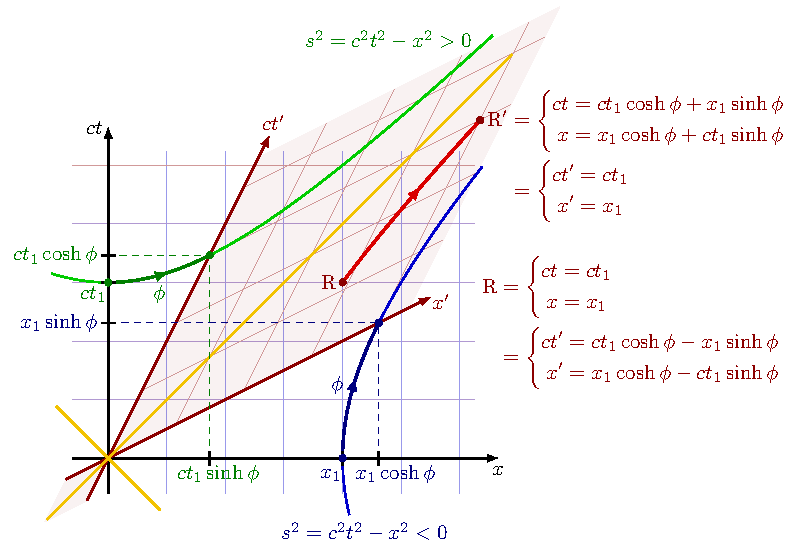
\includegraphics[width=0.9\linewidth]{figure/fig5.5}
	\caption[用双曲函数表示的洛伦兹变换方程]{用双曲函数表示的洛伦兹变换方程}
	\label{fig:fig5}
\end{figure}

\section{速度变换与低速极限}

由从 $K'$ 到 $K$ 的洛伦兹变换 \eqref{eq:ch5-standard-boost}
\[
x=\gamma(x'+Vt'),
\qquad
t=\gamma\left(t'+\frac{V}{c^{2}}x'\right)
\]
对无限小位移取差分，得到
\[
\dif x=\gamma(\dif x'+V\dif t'),
\]
\[
\dif t=\gamma\left(\dif t'+\frac{V}{c^{2}}\dif x'\right).
\]
因此
\[
v_{x}=\frac{\dif x}{\dif t}
=
\frac{\dif x'+V\dif t'}{\dif t'+\frac{V}{c^{2}}\dif x'}.
\]
分子分母同除以 $\dif t'$，可得纵向速度变换
\begin{equation}
\label{eq:ch5-longitudinal-velocity-transform}
v_{x}=
\frac{v'_{x}+V}{1+\frac{Vv'_{x}}{c^{2}}}.
\end{equation}

横向坐标满足 $\dif y=\dif y'$、$\dif z=\dif z'$，但时间微元仍按洛伦兹变换改变，因此
\begin{equation}
\label{eq:ch5-transverse-velocity-transform}
v_{y}=
\frac{v'_{y}}{\gamma\left(1+\frac{Vv'_{x}}{c^{2}}\right)},
\qquad
v_{z}=
\frac{v'_{z}}{\gamma\left(1+\frac{Vv'_{x}}{c^{2}}\right)}.
\end{equation}
\eqref{eq:ch5-longitudinal-velocity-transform} 和 \eqref{eq:ch5-transverse-velocity-transform} 说明，相对论中的速度叠加不是简单相加。

若 $v'_{x}=c$，则
\[
v_{x}=\frac{c+V}{1+\frac{V}{c}}=c.
\]
因此光速在 \eqref{eq:ch5-longitudinal-velocity-transform} 下仍保持为 $c$。当
\[
V\ll c,
\qquad
v'\ll c
\]
时，分母中的相对论修正项可以忽略，速度变换退化为伽利略速度叠加
\[
v_{x}\approx v'_{x}+V.
\]

\section{四维矢量}

在相对论中，一个四分量对象是否是四维矢量，不取决于它是否有四个分量，而取决于它在洛伦兹变换下是否满足规定的变换规律。若一个对象 $A^{\mu}$ 在洛伦兹变换下满足
\begin{equation}
\label{eq:ch5-four-vector-transform}
A'^{\mu}=\Lambda^{\mu}{}_{\nu} A^{\nu},
\end{equation}
则称满足 \eqref{eq:ch5-four-vector-transform} 的 $A^{\mu}$ 是反变四维矢量。

对应的协变分量仍由 \eqref{eq:ch5-lower-index} 给出。
由于洛伦兹变换保持度规不变，协变分量的变换可写为
\begin{equation}
\label{eq:ch5-covector-transform}
A'_{\mu}=\Lambda_{\mu}{}^{\nu} A_{\nu},
\end{equation}
\eqref{eq:ch5-covector-transform} 是协变四维矢量的变换规律。
其中
\[
\Lambda_{\mu}{}^{\nu}=\eta_{\mu\alpha}\Lambda^{\alpha}{}_{\beta}\eta^{\beta\nu}.
\]

四维矢量的内积 \eqref{eq:ch5-minkowski-inner-product} 是洛伦兹标量。即在任意惯性系中均有
\begin{equation}
\label{eq:ch5-inner-product-invariant}
A'^{\mu} B'_{\mu}=A^{\mu} B_{\mu}.
\end{equation}
\eqref{eq:ch5-inner-product-invariant} 正是四维矢量语言的核心优势：洛伦兹不变性可以通过指标缩并简洁表示。

常见的四维矢量包括事件坐标 $x^{\mu}$、位移 $\dif x^{\mu}$、四维波矢 $k^{\mu}$、四动量 $p^{\mu}$ 等。第六章将利用固有时定义四速度和四动量，从而把动力学方程写成洛伦兹协变形式。

\section{四维张量与反对称张量}

若一个二指标对象 $T^{\mu\nu}$ 在洛伦兹变换下满足
\begin{equation}
\label{eq:ch5-contravariant-tensor-transform}
T'^{\mu\nu}
=
\Lambda^{\mu}{}_{\alpha}\Lambda^{\nu}{}_{\beta}T^{\alpha\beta},
\end{equation}
则称满足 \eqref{eq:ch5-contravariant-tensor-transform} 的对象为二阶反变四维张量。若一个二指标对象 $T_{\mu\nu}$ 满足
\begin{equation}
\label{eq:ch5-covariant-tensor-transform}
T'_{\mu\nu}
=
\Lambda_{\mu}{}^{\alpha}\Lambda_{\nu}{}^{\beta}T_{\alpha\beta},
\end{equation}
则称满足 \eqref{eq:ch5-covariant-tensor-transform} 的对象为二阶协变四维张量。混合张量 $T^{\mu}{}_{\nu}$ 则有一个反变指标和一个协变指标，并按相应规则变换。

二阶张量可以按照指标交换性质分为对称部分和反对称部分。若
\[
S^{\mu\nu}=S^{\nu\mu},
\]
则称 $S^{\mu\nu}$ 为对称张量。若
\[
A^{\mu\nu}=-A^{\nu\mu},
\]
则称 $A^{\mu\nu}$ 为反对称张量。反对称张量的对角分量为零，因为令 $\mu=\nu$ 得
\[
A^{\mu\mu}=-A^{\mu\mu},
\]
从而
\[
A^{\mu\mu}=0.
\]
在四维时空中，二阶反对称张量有
\[
\frac{4\cdot 3}{2}=6
\]
个独立分量。这个结构在电动力学中非常重要，电磁场张量正是四维时空中的反对称二阶张量。

任意二阶张量均可分解为对称部分和反对称部分：
\begin{equation}
\label{eq:ch5-symmetric-antisymmetric-decomposition}
T^{\mu\nu}=T^{(\mu\nu)}+T^{[\mu\nu]},
\end{equation}
\eqref{eq:ch5-symmetric-antisymmetric-decomposition} 中
\begin{equation}
\label{eq:ch5-symmetrization}
T^{(\mu\nu)}=\frac{1}{2}(T^{\mu\nu}+T^{\nu\mu}),
\end{equation}
\begin{equation}
\label{eq:ch5-antisymmetrization}
T^{[\mu\nu]}=\frac{1}{2}(T^{\mu\nu}-T^{\nu\mu}).
\end{equation}
圆括号表示 \eqref{eq:ch5-symmetrization} 中的对称化，方括号表示 \eqref{eq:ch5-antisymmetrization} 中的反对称化。

\section{四维 Levi-Civita 张量与对偶}

为了处理四维时空中的完全反对称结构，引入四维排列符号 $[\mu\nu\rho\sigma]$，规定
\[
[0123]=1.
\]
若四个指标中有任意两个相同，则排列符号为零；交换任意两个指标时，排列符号变号。

需要注意，排列符号本身不是张量。四维 Levi-Civita 张量需要结合度规行列式定义。设
\[
g=\det(g_{\mu\nu}).
\]
在闵可夫斯基直角坐标中，
\[
g=\det(\eta_{\mu\nu})=-1,
\qquad
|g|=1.
\]
因此可取
\begin{equation}
\label{eq:ch5-levi-civita-definition}
\varepsilon^{\mu\nu\rho\sigma}
=
\frac{1}{\sqrt{|g|}}[\mu\nu\rho\sigma].
\end{equation}
\eqref{eq:ch5-levi-civita-definition} 在当前坐标中给出
\[
\varepsilon^{0123}=1.
\]
降低全部指标时，有
\[
\varepsilon_{\mu\nu\rho\sigma}
=
\eta_{\mu\alpha}\eta_{\nu\beta}\eta_{\rho\gamma}\eta_{\sigma\delta}
\varepsilon^{\alpha\beta\gamma\delta}.
\]
由于三个空间指标降低时各产生一个负号，所以
\[
\varepsilon_{0123}=-1.
\]
完全缩并满足
\[
\varepsilon^{\mu\nu\rho\sigma}\varepsilon_{\mu\nu\rho\sigma}=-4!=-24.
\]

对于反对称二阶张量 $A_{\rho\sigma}$，定义其对偶张量为
\begin{equation}
\label{eq:ch5-dual-antisymmetric-tensor}
{}^{*}A^{\mu\nu}
=
\frac{1}{2}\varepsilon^{\mu\nu\rho\sigma}A_{\rho\sigma}.
\end{equation}
\eqref{eq:ch5-dual-antisymmetric-tensor} 中系数 $1/2$ 用于去除反对称指标交换造成的重复计数。在四维时空中，二阶反对称张量的对偶仍是二阶反对称张量。该结构将在电磁场张量及其对偶张量中发挥核心作用。

\section{洛伦兹协变方程}

相对论要求物理定律在所有惯性系中具有相同形式。用四维张量语言，这一要求可以表述为洛伦兹协变性。若一个方程两边都是同类型四维张量，则该方程在洛伦兹变换下保持形式不变。

例如，若
\begin{equation}
\label{eq:ch5-vector-covariant-equation}
A^{\mu}=B^{\mu}
\end{equation}
在一个惯性系中成立，并且 $A^{\mu}$ 和 $B^{\mu}$ 都是四维矢量，则在另一个惯性系中有
\[
A'^{\mu}=\Lambda^{\mu}{}_{\nu} A^{\nu},
\qquad
B'^{\mu}=\Lambda^{\mu}{}_{\nu} B^{\nu}.
\]
由于 $A^{\nu}=B^{\nu}$，因此
\begin{equation}
\label{eq:ch5-transformed-vector-covariant-equation}
A'^{\mu}=B'^{\mu}.
\end{equation}
\eqref{eq:ch5-vector-covariant-equation} 变换为 \eqref{eq:ch5-transformed-vector-covariant-equation}，方程形式保持不变。

类似地，若
\[
T^{\mu\nu}=S^{\mu\nu}
\]
两边都是同类型二阶张量，则该方程也是洛伦兹协变的。若某个方程为标量方程，例如
\[
A^{\mu} A_{\mu}=\text{const},
\]
则其形式在所有惯性系中也保持不变。

因此，构造相对论性物理定律的基本策略是：把物理量组织为四维标量、四维矢量或四维张量，并使方程两边具有相同的张量类型。洛伦兹协变性不是额外装饰，而是狭义相对论中物理定律应当满足的基本结构要求。

\section{四维微分算符与达朗贝尔算子}

相对论场论中的场量依赖四维时空坐标。设标量场为
\[
\phi=\phi(x^{\mu}).
\]
定义四维偏导算符
\begin{equation}
\label{eq:ch5-partial-definition}
\partial_{\mu}=\frac{\partial}{\partial x^{\mu}}.
\end{equation}
\eqref{eq:ch5-partial-definition} 中由于 $x^{0}=ct$，所以
\[
\partial_{0}=\frac{\partial}{\partial x^{0}}=\frac{1}{c}\frac{\partial}{\partial t}.
\]
空间分量为
\[
\partial_{i}=\frac{\partial}{\partial x^{i}}.
\]
因此
\begin{equation}
\label{eq:ch5-four-gradient}
\partial_{\mu}=
\left(
\frac{1}{c}\frac{\partial}{\partial t},\bm{\nabla}
\right),
\end{equation}
其中
\[
\bm{\nabla}=
\left(
\frac{\partial}{\partial x},
\frac{\partial}{\partial y},
\frac{\partial}{\partial z}
\right).
\]
$\partial_{\mu}$ 是协变四梯度。升高指标得
\begin{equation}
\label{eq:ch5-raised-partial}
\partial^{\mu}=\eta^{\mu\nu}\partial_{\nu}.
\end{equation}
根据 \eqref{eq:ch5-raised-partial}，在当前号差约定下，
\begin{equation}
\label{eq:ch5-raised-four-gradient}
\partial^{\mu}=
\left(
\frac{1}{c}\frac{\partial}{\partial t},-\bm{\nabla}
\right).
\end{equation}

四维偏导的缩并给出达朗贝尔算子：
\begin{equation}
\label{eq:ch5-dalembertian-definition}
\dalembert =\partial^{\mu}\partial_{\mu}.
\end{equation}
\eqref{eq:ch5-dalembertian-definition} 展开为
\[
\dalembert =\eta^{\mu\nu}\partial_{\mu}\partial_{\nu}.
\]
由 \eqref{eq:ch5-four-gradient} 与 \eqref{eq:ch5-raised-four-gradient} 的具体形式可得
\begin{equation}
\label{eq:ch5-dalembertian-coordinate}
\dalembert =
\frac{1}{c^{2}}\frac{\partial^{2}}{\partial t^{2}}-\bm{\nabla}^{2}.
\end{equation}
\eqref{eq:ch5-dalembertian-coordinate} 是达朗贝尔算子在惯性直角坐标中的具体形式。
其中
\[
\bm{\nabla}^{2}=
\frac{\partial^{2}}{\partial x^{2}}
+
\frac{\partial^{2}}{\partial y^{2}}
+
\frac{\partial^{2}}{\partial z^{2}}.
\]
达朗贝尔算子是洛伦兹标量算符。相对论性波动方程可以写为
\begin{equation}
\label{eq:ch5-relativistic-wave-equation}
\dalembert \phi=0.
\end{equation}
展开后为
\[
\frac{1}{c^{2}}\frac{\partial^{2}\phi}{\partial t^{2}}-\bm{\nabla}^{2}\phi=0.
\]
\eqref{eq:ch5-relativistic-wave-equation} 这种四维形式直接显示了方程的洛伦兹协变性。

在惯性直角坐标中，闵可夫斯基度规为常数，因此普通偏导可以直接用于四维张量场。若采用一般曲线坐标或弯曲时空坐标，则需要用协变导数替代普通偏导。本章只讨论狭义相对论中的惯性坐标。

\section{本章小结}

本章建立了狭义相对论的四维时空语言。狭义相对论以相对性原理和光速不变原理为基础，要求时间与空间统一为四维闵可夫斯基时空。事件的坐标写为
\[
x^{\mu}=(ct,x,y,z),
\]
时空间隔为
\[
\dif s^{2}=\eta_{\mu\nu}\dif x^{\mu}\dif x^{\nu},
\qquad
\eta_{\mu\nu}=\mathrm{diag}(1,-1,-1,-1).
\]

固有时由类时世界线的间隔定义：
\[
c^{2}\dif\tau^{2}=\dif s^{2}.
\]
它是沿粒子世界线自身测得的时间，也是后续建立相对论力学的自然参数。

洛伦兹变换是保持闵可夫斯基度规的线性变换，其矩阵满足
\[
\Lambda^{T}\eta\Lambda=\eta.
\]
所有满足这一条件的实线性变换构成洛伦兹群 $O(1,3)$。沿一维方向的 boost 可以表示为闵可夫斯基平面中的双曲旋转，快度 $\theta$ 满足
\[
\tanh\theta=\frac{V}{c}.
\]

四维矢量和四维张量的定义由洛伦兹变换规律给出。四维矢量满足
\[
A'^{\mu}=\Lambda^{\mu}{}_{\nu} A^{\nu},
\]
二阶反变张量满足
\[
T'^{\mu\nu}=
\Lambda^{\mu}{}_{\alpha}\Lambda^{\nu}{}_{\beta}T^{\alpha\beta}.
\]
通过闵可夫斯基度规可以升降指标，并构造洛伦兹标量。

反对称二阶张量在四维时空中有六个独立分量。借助四维 Levi-Civita 张量，可以定义反对称二阶张量的对偶：
\[
{}^{*}A^{\mu\nu}
=
\frac{1}{2}\varepsilon^{\mu\nu\rho\sigma}A_{\rho\sigma}.
\]
该结构为后续电磁场张量的四维表达做准备。

四维偏导算符为
\[
\partial_{\mu}=
\left(
\frac{1}{c}\frac{\partial}{\partial t},\bm{\nabla}
\right),
\]
升高指标后为
\[
\partial^{\mu}=
\left(
\frac{1}{c}\frac{\partial}{\partial t},-\bm{\nabla}
\right).
\]
由此得到达朗贝尔算子
\[
\dalembert =\partial^{\mu}\partial_{\mu}
=
\frac{1}{c^{2}}\frac{\partial^{2}}{\partial t^{2}}-\bm{\nabla}^{2}.
\]

本章的核心思想是：相对论性物理定律应写成洛伦兹协变形式。也就是说，方程两边应具有相同的四维张量类型，或共同构成洛伦兹标量。这样，方程一旦在一个惯性系中成立，就会在所有惯性系中保持相同形式。下一章将在本章时空结构的基础上，引入四速度、四动量和四力，从而建立相对论力学。
